\clearpage
\newpage
\section{Przechowywanie i transmisja danych}
\label{sec:przesyl}

\subsection{GIS}
\label{subsec:gis}

GIS(Geographical Information Systems) jest to System Informacji Geograficznych, połącznie danych i technologi aby dokonywać pomiarów, analizy i przedstawiania danych związanych z informacjami geograficznymi. Dane są pobieranie w trakcie naziemnych pomiarów jak i zbierane przy użyciu sztucznych satelitów. Informacje te są następnie zapisywane do określonych formatów dzięki czemu możliwe jest ich dalsze przetwarzanie.

\subsubsection{Wykorzystywany układ współrzędnych}
\label{subsec:uklad}

Istnieje wiele układów współrzędnych które służą do opisu pojedyńczego punktu na powierzchni ziemi. Na stronie \underline{\texttt{http://www.spatialreference.org/ref/epsg/}} (dostęp 20.08.2013) znajduje się lista zawierająca przykłady zapisu punktu na kuli ziemskiej przy użyciu różnych formatów, zawierają one niezbędne infomacje do poprawnego zapisu danych w określonym formacie.

Tradycyjny zapis oparty jest na wykorzystaniu stopni, minut i sekunk, jest on obecnie wypierany przez nowszy, łatwiejszy do obliczeń komputerówych. Wersją która ma za zadanie być ogólnoświatowym formatem jest WGS(World Geodetic System). Jego ostatnia wersja  WSG84 jest powszechnie używana w urządzeniach do nawigacji. Poniżej zaprezentowano jak wygląda zapis w starszym i nowszym punktu określającego położenie budynku A-0 uczelni AGH.

\begin{itemize}

\item
Pierwotny zapis

50°03'52.2803", 019°55'23.7968"
\item
Zapis unowocześniony

50.06452231874906, 19.923276901245117
\end{itemize}

Drugi zapis został wykorzystany do przechowywania danych w plikach, tak aby wymiana i wspólna praca była jak najprostsza. Wybór ten sprawił że nie występuje problem konwersji punktu do formatu czytelnego dla komputera, można go bez problemu odczaytać jako liczbę.

\subsection{Format zapisu}
\label{subsec:zapisWektorowy}

W celu przechowywania obiektów graficznych zdecydowano się na wykorzystanie grafiki wektorowerj. Oprócz bezproblemowej skalowalności, pozwala ona również na szeroką i łatwą edycję.
Obraz jest w tym przypadku przechowywany jako zbiór formuł matematycznych m.in. proste i łuki. Dzięki takiemu podejściu obraz w dowolnej skali na identyczną jakość, widać to na rysunku \ref{fig:wekt}. Przykładowymi formatami są GML(Geography Markup Language) otwarty standart XML dla wymiany danych GIS, Shapefile czy tradycyjny kartezjański układ współrzędnych.

  \begin{figure}[H]
  \centering
    
\includegraphics[width=50mm]{ge/a1.jpg}
  \caption{Zapis wektorowy}
  \label{fig:wekt}
  \end{figure}

Przeciwnym podejściem jest grafika rastrowa, jest to zapis punktów o określonym kolorze i położeniu na płaszczyźnie.  Efektem takiego podejścia jest pogorszenie obrazu w momencie dużego powiększenia. Przykładem są formaty takie jak ADRG,ASC czy RGB.
Porównanie litery a i jej 7-krotnego powiększenia w tym zapise zaprezentowano na rysunku \ref{fig:rast}
  \begin{figure}[H]
  \centering
    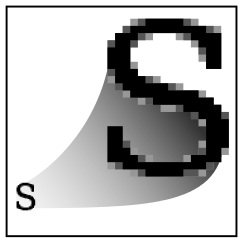
\includegraphics[width=50mm]{ge/a2.jpg}
  \caption{Zapis rastrowy}
  \label{fig:rast}
  \end{figure}

\subsection{Format pliku}
\label{subsec:fileformat}

W celu wypełnienia założeń projektu jakim jest umożliwienie przechowywania danych w zewnętrznym pliku przeprowadzono analizę dostępnych foramtów zapisu danych kartograficznych.

\begin{itemize}

\item
SWDE(Standard Wymiany Danych Ewidencyjnych) - polski format służący głównie do wymiany danych ewidencyjnych gruntów i budynków

\item
SWING(Standard Wymiany INformacji Geodezyjnych) - format danych geodezyjnych służący do wymiany danych pomiędzy bazami danych systemów informatycznych SIT(wikipedia.pl)

\item
KML(Keyhole Markup Language) - otwarty standart oparty na XML-u, stworzony głównie dla potrzeb GoogleEarth

\item
GML(Geography Markup Language) - stworzony przez OGC(Open Geospatial Consortium) międzynarodową organizację założoną w celu tworzenia i rozpowszechniania standarów związanych z informacjami dotyczącymi geograficznych i geoprzestrzennych danych

\end{itemize}

Dwa polskie formaty są stosunkowo mało popularne, są one głównie wykorzystywane w celu kompunikacji pomiędzy rządowymi bazami danych. Zawierają one bardzo określone typy danych co sprawia że są mało przydatne dla omawianego projetku. KML jest foramtem który posiada szeroki wachlarz dostępnych znaczników a jego duża popularność dostarcza dużą bazę plików gotowych do wykorzystania. Niestety został on stworzony by współpracować z określonym programem, zaimplementowane zostały jedynie elementy które mogą zostać wykorzystane w nim. Ostani przykład został stworzony w uniwersalnym celu do ogólnego użytku, posiada on bardzo dużo możliwości, apadtacji do konkretnych rozwiązań\cite{gml} z uwagi na ten fakt zdecydowano się na wybór tego rozwiąznia. Nie zostaną wykorzystane jego pełne możliwości, jedynie te które są przydatne w projektowanej aplikacji.
Jedną z ciekawych i przydatnych możliwości podczas jego wykorzystania jest zgodność z formatem KML na bazie którego powstało wiele zbiorów danych gotowych do wykorzystania.

\subsection{Parser plików}
\label{subsec:parser}

Założenia projektu zakładają dostarczanie wstępnego zestawu danych opisujących mapę poprzez plik tekstowy zawierający dane w okrślonym formacie. Może on znajdować się na zewnętrznym serwerze lub dysku lokalnym. W pierwszym przypadku zostanie on najpierw ściągnięty do pamięci lokalnej aby następnie mógł być wykorzystany, w drugim po podaniu ścieżki dostępu do niego  od razu nastąpi jego analiza. Aby było to możliwe stworzony został parser którego zadaniem jest odczytanie danych i przygotowanie ich aby możliwe było ich wykorzystanie w dalszej pracy aplikacji.
Wybrany format danych wybrany podczas prac badawczych, GML, zawiera bardzo obszerny zbiór elementów pozwalających opisywać bardzo szeroki wachlarz obiektów, takich jak mosty, budynki pojazdy. Taka dokładność nie jest wymagana w tym przypadku z tego powodu parser nie obsługuje całego języka. Ponieważ można przygotować plik w formacie GML w taki sposób aby przypominał zapis KML zdecydowano się zwrócić szczgólną uwagę aby parser poprawnie rozpoznawał i dekodował dane również z tej postaci, pozwoli to na dostęp do dużej bazy gotowych informacji.
Wczytane informacje podlegają przetworzniu ze składni XML, na którym bazuje GML do notacji JSON która jest używana podczas pracy map.

\subsection{Storage}
\label{subsec:storage5}
Aby stworzyć framework któy będzie w stanie działać przy minimalnej konieczności konfiguracji dodatkowych środowisk postanowiono aby dane w pierwszej kolejności były przechowywane po stronie klienta. Do tego celu nadaje się funkcjonalność stworzona w ostatniej wersji HTML którą jest Storage. Pozwala on na przechowywanie danych w przeglądarce użytkownika \cite{html5dive}. Różnicą w stosunku do ciasteczek które również potrafią przechowywać dane są:
\begin{itemize}
\item
Większy rozmiar dostępnej pamięci m.in. Chrome 5MB \nocite{chrome5mb}, IE 10MB
\item
Informacje przechowywane są po stronie użytkownka, nie są przesyłane za każdym razem do serwera.
\item
Informacja może być przechowywana przez długi okres czasu.
\end{itemize}

Wadą tego typu pamięci jest jej interfejs. Obecnie przechowywany sposób danych to mapowanie w postaci napis->napis. Wymusza to aby dane które chcemy przechować były zapisane jako ciągi znaków. Przykład \ref{lis:storage} przedstawia w jaki sposób możemy obiekt zawierający imię i nazwisko zapisać w pamięci. Linia 4 przedstawia obiekt w postaci której chcielibyśmy go przechować. Niestety zwykłe przypisanie do zmiennej w pamięci powoduje że jedynie typ instancji zostaje zapisany. Aby móc zapisać w poprawnej formie dane musimy doknać serializacji danych. Czynność tą możemy wykonać przy pomocy metody stringify z obiektu JSON, wynikiem jest ciąg znaków który możemy bez problemu zapisać w pamięci sesyjnej. Do odzyskania pierwotnego obiektu, odtworzenia go z zapisanego napisu wykorzystujemy metodę parse również z obiektu JSON.

Dodatkowo nie można pominąć faktu istnienia dwóch typów.
\begin{itemize}

\item
Session Storage

Dane przechowywane są w kontekście sesji użytkownika, są one tracone w momencie zamknięcia okna przeglądarki.

\item
Local Storage

Teoretycznie dane są przechowywane w nieskończoność, do momentu kiedy użytkonwik nie usunie ich. Zamknięcię sesji nie powoduje usunięcia danych.

\end{itemize}

Zapisywanie informacji po stronie klienta ma na celu zachowanie aktualnego stanu mapy, dokonanych zmian i naniesionych poprawek, informacje o poprzednich są zbędne. Sytuacja ta jednoznacznie wskazuje że lepszym wyborem jest pamięć sesyjna(Session Storage).

\lstset{language=JavaScript}
\label{lis:storage}
\begin{lstlisting}[caption=json]
      uzytkownik={};
      uzytkonwik.imie='Jan'
      uzytkownik.nazwisko='Kowalski'
      //uzytkownik : Object {imie: "Jan", nazwisko: "Kowalski"}

      sessionStorage.u1 = uzytkownik
      //sessionStorage.u1 : "[object Object]"

      sessionStorage.u2 = JSON.stringify(uzytkownik)
      //sessionStorage.u2 : "{"imie":"Jan","nazwisko":"Kowalski"}"

      uzytkonwik2 = JSON.parse(sessionStorage.u2)
      //uzytkonwik2 : Object {imie: "Jan", nazwisko: "Kowalski"}
\end{lstlisting}


Podsumowanie dostępne na stornie \underline{\texttt{http://www.html5rocks.com/en/features/storage}}(dostęp 31.10.2013) pozwala na sprawdzenie minimalnej wersji przęglądarki od której wspierane jest to rozwiązanie. Wskazuje ono na największą dostępność spośród ponadych sposobów przechowywania informacji po stornie klienta.

\subsection{Transmisja danych}
\label{subsec:transmisjaDanych}

Ważnym aspektem który należy rozwiązać jest sposób przesyłania danych. Problem ten jest szczególnie istotny w omawianej pracy z uwagi na możliwość przesyłania dużej ilości informacji o granicach lub innych liniach przezentowanych na mapie. Do opisu kwadratowego obszaru wymagane jest przesłanie informacji o minimum 4 punktach. Jeżeli będziemy chcieli przekazać dokłądniejszy zarys obszaru, zaprezentować granicę państwa lub linię frotnu wojennego linia prosta w większości przypadków będzie zbyt ogólnym przybliżeniem, nie oddającym prawdziwej sytuacji.

Projekt zakłada korzystanie z lokalnej pamięci komputera użytkownika podczas pracy, jednak dostarczenie informacji, danych wejściowych nie powinno być ograniczone do wczytania ich z pliku tekstowego, należy pamiętać o możliwości przesłania ich z serwera aplikacji do użytkownika. W sytuacji takiej, gdzie w jednym momencie przesłane zostaną wszystkie informacje dotyczące mapy, ilość danych może być znaczna.

Z raportu Akamai wynika że śrenia przepływność łączy internetowych dla użytkowników korzystających z puli adresów IP przeznaczonych dla Polski w I kwartale 2012 r. wynosiła 5Mb/s  \underline{\texttt{http://www.rp.pl/artykul/924483.html}} (dostęp 13.04.2014). Jest to bardzo dobry wynik który plasuje Polskę w czołówce rankingu. Pomimo tegowyniku nie można pominąć faktu optymalizacji przesyłanych danych, wymieniane dane pomiędzy użytkownikiem a serwerem powinny być jak najmniejsze. Duża popularność urządzeń mobilnych w których dostęp do internetu jest zapewniany często poprzez sieć bezprzewodową a dostęp do interentu nie jest jeszcze tak dogodny jak jest to w przypadku użytkowników stacjonarnych  wymusza minimalizowanie przesyłanych informacji.

Kolejnym powodem dla którego odpowiedzi serwera powinny być jak najlżesze jest koszt pracy samego serwera. Jest to szczególnie widoczne w dużych aplikacjach mających wielu użytkowników, czas jaki jest przeznaczany dla pojedyńczego jest mnożony przez ich ilość. Z tego powodu zawsze podczas zwiększenia ilości użtkowników korzystających z aplikacji następuje zwiększenie stawianych wymagać wobec serwera, w ostateczności wymagane jest wykorzystanie kolejnej fizycznej maszyny. Celem programisty tworzącego kod który będzie wykorzystywał zasoby serwera(zarówno jego czas procesora jak i pamięć) jest dbanie aby moment w którym niezbędne będzie korzystanie z większej ilośći maszym nastąpił przy jak największej ilości użytkowników.

Z uwagi na omówione aspekty zdecydowano się aby w przypadku korzystania z danych nie znajdujacych się na lokalnym dysku komputera wszystkie infromacje dotyczące mapy zostały przesłane jako plik w określonym formacie. Zostałby on zapisany w pamięci komputera użytkownika i podlegał dalszej pracy. Takie podejście minimalizuje wymagania nakładane na serwer i czas zajęcia procesowa.

\newpage
